\documentclass[
	12pt,
	a4paper,
	bibtotoc,
	cleardoubleempty, 
	idxtotoc,
	ngerman,
	openright
	final,
	listof=nochaptergap,
	]{scrbook}

\usepackage[utf8]{inputenc}
\usepackage[T1]{fontenc}

% ##################################################
% Unterstuetzung fuer die deutsche Sprache
% ##################################################
\usepackage {ngerman}
\usepackage[ngerman] {babel}
%\usepackage{url}
\newcommand\myworries[1]{\textcolor{red}{#1}}
% ##################################################
% Dokumentvariablen
% ##################################################

% Persoenliche Daten
\newcommand{\docNachname}{Jan Stodt} 
\newcommand{\docVorname}{Axel Butz, Eugen Jastremskoj, Marcin Krawczyk, Jan Ondruch,}
\newcommand{\docStrasse}{255358 (Jan O) (Brno University of Technology(VUT))}
\newcommand{\docOrt}{}
\newcommand{\docPlz}{}
\newcommand{\docEmail}{}
\newcommand{\docMatrikelnummer}{227712(Ax) 247725(Eu) 246286(Jan S) 248667(Mar)}

% Dokumentdaten
\newcommand{\docTitle}{Med-Eval}
%\newcommand{\docUntertitle}{} % Kein Untertitel
\newcommand{\docUntertitle}{Medizinisches Evaluationssystem in Kooperation mit Uniklinik Freiburg - Deutsche Telekom}
% Arten der Arbeit: Bachelorthesis, Masterthesis, Seminararbeit, Diplomarbeit
\newcommand{\docArtDerArbeit}{Projektarbeit}
%Studiengaenge: Allgemeine Informatik Bachelor, Computer Networking Bachelor,
% Software-Produktmanagement Bachelor, Advanced Computer Scinece Master
\newcommand{\docStudiengang}{Computer Networking Bachelor}
\newcommand{\docAbgabedatum}{17.02.2017}
\newcommand{\docErsterReferent}{Prof. Dr. Achim P. Karduck}
%\newcommand{\docZweiterReferent}{-} % Wenn es nur einen Betreuer gibt
\newcommand{\docZweiterReferent}{-}

% ##################################################
% Allgemeine Pakete
% ##################################################

% Abbildungen einbinden
\usepackage{graphicx}

% Zusaetsliche Sonderzeichen
\usepackage{dingbat}

% Farben
\usepackage{color}
\usepackage[usenames,dvipsnames,svgnames,table]{xcolor}

% Maskierung von URLs und Dateipfaden
\usepackage[hyphens]{url}

% Deutsche Anfuehrungszeichen
\usepackage[babel, german=quotes]{csquotes}

% Pakte zur Index-Erstellung (Schlagwortverzeichnis)
\usepackage{index}
\makeindex

% Ipsum Lorem
% Paket wird nur für das Beispiel gebraucht und kann gelöscht werden
\usepackage{lipsum}

% ##################################################
% Seitenformatierung
% ##################################################
\usepackage[
	portrait,
	bindingoffset=1.5cm,
	inner=2.5cm,
	outer=2.5cm,
	top=3cm,
	bottom=2cm,
	%includeheadfoot
]{geometry}

% ##################################################
% Kopf- und Fusszeile
% ##################################################

\usepackage{fancyhdr}

\pagestyle{fancy}
\fancyhf{}
\fancyhead[EL,OR]{\sffamily\thepage}
\fancyhead[ER,OL]{\sffamily\leftmark}

\fancypagestyle{headings}{}

\fancypagestyle{plain}{}

\fancypagestyle{empty}{
	\fancyhf{}
	\renewcommand{\headrulewidth}{0pt}
}

%Kein "Kapitel # NAME" in der Kopfzeile
\renewcommand{\chaptermark}[1]{
	\markboth{#1}{}
	\markboth{\thechapter.\ #1}{}
}

% ##################################################
% Schriften
% ##################################################

% Stdandardschrift festlegen
\renewcommand{\familydefault}{\sfdefault}

% Standard Zeilenabstand: 1,5 zeilig
\usepackage{setspace}
\onehalfspacing 

% Schriftgroessen festlegen
\addtokomafont{chapter}{\sffamily\large\bfseries} 
\addtokomafont{section}{\sffamily\normalsize\bfseries} 
\addtokomafont{subsection}{\sffamily\normalsize\bfseries} 
\addtokomafont{caption}{\sffamily\normalsize\mdseries} 

% ##################################################
% Inhaltsverzeichnis / Allgemeine Verzeichniseinstellungen
% ##################################################

\usepackage{tocloft}

% Punkte auch bei Kapiteln
\renewcommand{\cftchapdotsep}{3}
\renewcommand{\cftdotsep}{3}

% Schriftart und -groesse im Inhaltsverzeichnis anpassen
\renewcommand{\cftchapfont}{\sffamily\normalsize}
\renewcommand{\cftsecfont}{\sffamily\normalsize}
\renewcommand{\cftsubsecfont}{\sffamily\normalsize}
\renewcommand{\cftchappagefont}{\sffamily\normalsize}
\renewcommand{\cftsecpagefont}{\sffamily\normalsize}
\renewcommand{\cftsubsecpagefont}{\sffamily\normalsize}

%Zeilenabstand in den Verzeichnissen einstellen
\setlength{\cftparskip}{.5\baselineskip}
\setlength{\cftbeforechapskip}{.1\baselineskip}

% ##################################################
% Abbildungsverzeichnis und Abbildungen
% ##################################################

\usepackage{caption}

\usepackage{wrapfig}

% Nummerierung von Abbildungen
\renewcommand{\thefigure}{\arabic{figure}}
\usepackage{chngcntr}
\counterwithout{figure}{chapter}

% Abbildungsverzeichnis anpassen
\renewcommand{\cftfigpresnum}{Abbildung }
\renewcommand{\cftfigaftersnum}{:}

% Breite des Nummerierungsbereiches [Abbildung 1:]
\newlength{\figureLength}
\settowidth{\figureLength}{\bfseries\cftfigpresnum\cftfigaftersnum}
\setlength{\cftfignumwidth}{\figureLength}
\setlength{\cftfigindent}{0cm}

% Schriftart anpassen
\renewcommand\cftfigfont{\sffamily}
\renewcommand\cftfigpagefont{\sffamily}

% ##################################################
% Tabellenverzeichnis und Tabellen
% ##################################################

% Nummerierung von Tabellen
\renewcommand{\thetable}{\arabic{table}}
\counterwithout{table}{chapter}

% Tabellenverzeichnis anpassen
\renewcommand{\cfttabpresnum}{Tabelle }
\renewcommand{\cfttabaftersnum}{:}

% Breite des Nummerierungsbereiches [Abbildung 1:]
\newlength{\tableLength}
\settowidth{\tableLength}{\bfseries\cfttabpresnum\cfttabaftersnum}
\setlength{\cfttabnumwidth}{\tableLength}
\setlength{\cfttabindent}{0cm}

%Schriftart anpassen
\renewcommand\cfttabfont{\sffamily}
\renewcommand\cfttabpagefont{\sffamily}

% Unterdrueckung von vertikalen Linien
\usepackage{booktabs}

% ##################################################
% Listings (Quellcode)
% ##################################################

\usepackage{listings}
\lstset{
	language=java,
	backgroundcolor=\color{white},
	breaklines=true,
	prebreak={\carriagereturn},
	breakautoindent=true,
	numbers=left,
	numberstyle=\tiny,
	stepnumber=2,
	numbersep=5pt,
	keywordstyle=\color{blue},
	commentstyle=\color{green},   
	stringstyle=\color{gray}
}
  	
% ##################################################
% Theoreme
% ##################################################
  	
% Umgebung fuer Beispiele
\newtheorem{beispiel}{Beispiel}

% Umgebung fuer These
\newtheorem{these}{These}

% Umgebung fuer Definitionen
\newtheorem{definition}{Definition}
  	
% ##################################################
% Literaturverzeichnis
% ##################################################

\usepackage{bibgerm}

% ##################################################
% Abkuerzungsverzeichnis
% ##################################################

\usepackage[printonlyused]{acronym}

% ##################################################
% PDF / Dokumenteninternelinks
% ##################################################
\usepackage{float}
\usepackage{textcomp}

\usepackage[
	colorlinks=false,
	linkcolor=black,
	citecolor=black,
	filecolor=black,
	urlcolor=black,
	bookmarks=true,
	bookmarksopen=true,
	bookmarksopenlevel=3,
	bookmarksnumbered,
	plainpages=false,
	pdfpagelabels=true,
	hyperfootnotes,
	pdftitle ={\docTitle},
	pdfauthor={\docVorname~\docNachname},
pdfcreator={\docVorname~\docNachname}]{hyperref}

\begin{document}

\setcounter{secnumdepth}{3}

% Titelblatt
\begin{titlepage}
	\pagestyle{empty}
		
	% ##################################################
	% HFU-Logo einbinden
	% ##################################################
	\begin{flushright}
		\begin{figure}[ht]
			\flushright
			
\includegraphics[height=3cm]{content/pictures/hfu.jpg}
		\end{figure}
	\end{flushright}
		
	% ##################################################
	% Titel
	% ##################################################
	\begin{center}
		{\fontsize{18}{22} \selectfont \docArtDerArbeit}\\[5mm]
		{\fontsize{18}{22} \selectfont im Studiengang} \\[5mm]
		{\fontsize{18}{22} \selectfont \docStudiengang}\\
		\vspace{1cm}
		\begin{onehalfspace}
			{\fontsize{22}{26} \selectfont \textbf{\docTitle}}\\[5mm]
			{\fontsize{18}{22} \selectfont \docUntertitle}
						
						
		\end{onehalfspace}
	\end{center}
		
	% ##################################################
	% Zusatzinformationen
	% ##################################################
	\vfill
	\begin{center}
		\begin{tabular}{lcl}
			Referent      & : & \docErsterReferent                 \\ \\
			Koreferent    & : & \docZweiterReferent                \\ \\	
			Vorgelegt am  & : & \docAbgabedatum                    \\ \\
			Vorgelegt von & : & \docVorname~\docNachname           \\
			              &   & Matrikelnummer: \docMatrikelnummer \\
			              &   & \docStrasse,~\docPlz~\docOrt       \\
			              &   & \docEmail                          
		\end{tabular}
	\end{center}
\end{titlepage}
\cleardoubleemptypage

\frontmatter

\lstdefinestyle{myCustomSmallSizeStyle}{
  language=Matlab,
  numbers=left,
  stepnumber=1,
  numbersep=10pt,
  tabsize=4,
  showspaces=false,
  showstringspaces=false
}

\lstdefinelanguage{JavaScript}{
  keywords={typeof, new, true, false, catch, function, return, null, catch, switch, var, if, in, while, do, else, case, break},
  keywordstyle=\color{blue}\bfseries,
  ndkeywords={class, export, boolean, throw, implements, import, this},
  ndkeywordstyle=\color{darkgray}\bfseries,
  identifierstyle=\color{black},
  sensitive=false,
  comment=[l]{//},
  morecomment=[s]{/*}{*/},
  commentstyle=\color{purple}\ttfamily,
  stringstyle=\color{red}\ttfamily,
  morestring=[b]',
  morestring=[b]"
}

% Abstract
\chapter*{Abstract\markboth{Abstract}{}}
\addcontentsline{toc}{chapter}{Abstract}
% english abstract
In the \textbf{Med-Eval} project, a cloud-based web application was created to support clinical trial surveys.
Med-Eval is based on an open-source survey tool which has been adapted for the use in clinical environments. The survey tool allows a modular set-up system to be configured for the creation of the questionnaires. The orchestration of the survey system is handled by the Open Source Tools Ansible.

\hfill \break

%german abstract
%keine Einrückung -> \noindent
\noindent
Im Projekt \textbf{Med-Eval} wurde eine Cloud gestützte Web-Applikation für die Unterstützung der Umfragen von klinischen Studien erstellt.
Med-Eval basiert auf einem Open-Source Umfragetool welches für die Verwendung in klinischem Umfeld angepasst wurde. Durch das Umfragetool ist ein modulares Baukasten-System für die Erstellung der Fragebögen konfigurierbar. Die Orchestrierung des Umfragesystems erfolgt mittels dem Open Source Tools Ansible.
\cleardoubleemptypage

% Inhaltsverzeichnis
\tableofcontents
\addcontentsline{toc}{chapter}{Inhaltsverzeichnis}
\cleardoubleemptypage

% Abbildungsverzeichnis einbinden und ins Inhaltsverzeichnis
% WORKAROUND: tocloft und KOMA funktionieren zusammen nicht
% korrekt\phantomsection
\addcontentsline{toc}{chapter}{\listfigurename} 
\listoffigures
\cleardoubleemptypage

% Tabellenverzeichnis einbinden und ins Inhaltsverzeichnis
% WORKAROUND: tocloft und KOMA funktionieren zusammen nicht
% korrekt\phantomsection
\phantomsection
\addcontentsline{toc}{chapter}{\listtablename}
\listoftables
\cleardoubleemptypage

% Abkürzungsverzeichnis
\chapter*{Abkürzungsverzeichnis\markboth{Abkürzungsverzeichnis}{}}
\addcontentsline{toc}{chapter}{Abkürzungsverzeichnis}

\begin{acronym}
		
%	\acro{SDN}{Software Defined Networking}

		
		
		
\end{acronym}

\phantomsection
\addcontentsline{toc}{chapter}{\lstlistlistingname}
\lstlistoflistings
\cleardoubleemptypage


\mainmatter

%add chapters here
\chapter{Einleitung}
Im Projekt Med-Eval ist eine Web-Applikation für die Unterstützung
von klinischen Studien entstehen. 
Studienteilnehmer/innen sollen per QR-Code den Link zum Studien-
Fragebogen öffnen. Die Navigation durch den Fragebogen soll auf dem Endgerät
(Laptop/Smartphone) schrittweise erfolgen, und lokal überprüft sein.
Die Daten kann jederzeit vom Server abgerufen werden, für eine später Auswertung.
Wir nutzen hierfür das Open Source Tool Limesurvey, welches wir für die
medizinische Umgebung angepasst haben.
Die Verbindung bei einer Umfrage und Abruf der Daten werden über SSL gesichert werden.
Auch der Server ist gegen die gängigsten Angriffsarten abgesichert.
Die Software kann durch das Ansible Deployment System auf jeden beliebigen Server, welcher die Voraussetzungen erfüllt,
innerhalb von kurzer Zeit installiert werden.
Limesurvey ist ein modulares Baukasten-System für die Erstellung der Fragebögen konfigurierbar.
Wir haben es um einen weitere Fragetyp, welche es einem Teilnehmer einer Umfrage ermöglicht
ein oder mehrere Körperteile anzugeben.
Des weiteren haben wir eine Möglichkeit erarbeitet einer Umfrage Umweltdaten wie Wetter und Mondstand
hinzufügen basierend auf dem Standort des Umfrageteilnehmers. Dies Daten können im Zusammenhang mit der Wirksamkeit eines
Medikaments eine Rolle spielen.
Die Umfrage sollte auf Desktop sowie gängigen Smartphone nutzbar sein.

\begin{figure}[!ht]
\centering
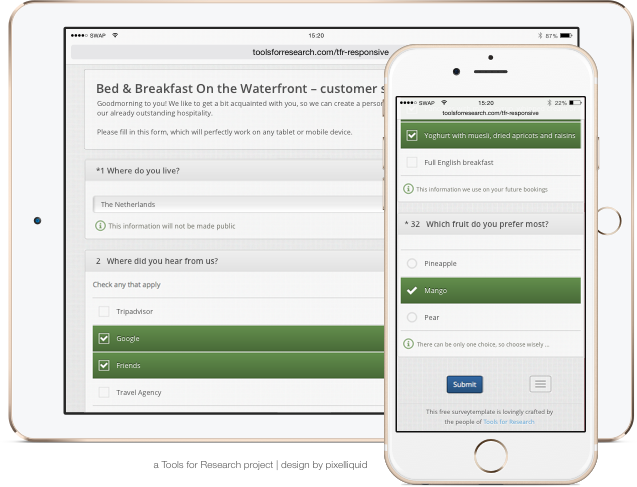
\includegraphics[width=0.6\textwidth]{content/pictures/preview.png}
\caption{Beispiel Desktop and Mobile Umfrage}
\url{https://www.toolsforresearch.com/sites/toolsforresearch.com/files/preview.png}
\label{fig_holo3}
\end{figure}



\chapter{Grundlagen}
% Grundlagen limesurey
% Grundlagen Erweiterung des limesurvey
% Grundlagen Linux Server Verwalung
% Grundlagen Ansible
% Grundlagen Hardening
Soll das Projekt Med-Eval in zukünftigen Semesterprojekten oder Thesis Arbeiten erweitert werden, sollte zunächst die derzeit verwendeten Technologien betrachtet werden. Diese sind eine essenzielle Anforderung an die Studenten/innen.

\section{Kenntnisse und Fähigkeiten}
Eine zentrale Fähigkeit, welche für die Weiterführung benötigt wird, ist die Fähigkeit Server Systeme (ohne Grafische Oberfläche) installieren, bedienen sowie warten zu können. Diese Fähigkeit wird bereits im ersten Semester vermittelt. Zudem ist es sehr Ratsam sich mit der Orchestrierungssoftware Ansible vertraut zu machen. Diese Software ermöglicht es den Anwender schnell und mit wenig Aufwand vorkonfigurierte Abläufe neu deployen zu können. Die Platform Med-Eval wurde vollständig mittels Ansible automatisiert. 
Ratsam wäre zudem die Fähigkeit Risiken einer Software zu ermitteln und geeignete Gegenmaßnahmen ergreifen zu können. Hierbei kann jedoch in dem meisten Fällen auf Informationen im Internet zugriffen werden.
Weiterhin wäre es sehr ratsam sich mit Script Sprachen der Webentwicklung wie JavaScript oder Node.js vertraut zu machen, bzw. dort bereits Vorkenntnisse vorweisen zu können. Des weitern 2 Erweiterungen auf Systemebene mit Python geschrieben, weshalb es ratsam ist sich grundlegende Kenntnisse von Python anzueignen.

\section{Projektunterstützende Maßnahmen}
Soll das Projekt erfolgreich abgeschlossen werden, ist es Ratsam Projektunterstützende Maßnahmen zu ergreifen. Dies umfasst die Verwendung einer Versionsverwaltung zu nützen \url{https://github.com}. So können parallel Code Änderungen vorgenommen werden, eine Vollständige Historie des Codes erhalten so wie gezielt neue Funktionen in das existierende System aufgenommen werden.
Neben der Code Verwaltung ist ein weiterer wichtiger Punkt die Team Kommunikation. Diese sollte einfach und schnell umsetzbar sein. Um dies zu erreichen, kann auf die Teamkommunikationssoftware Slack \url{https://slack.com} genutzt werden. Diese Software wurde erfolgreich in Firmen und Organisationen wie der NASA sowie IBM erprobt.
\\
\section{Entwicklungsprozess}
Um einen möglichst reibungslosen Entwicklungsprozess zu erreichen sollte auf die Entwicklungskonzepte Test getriebene Entwicklung oder Agile zurückgegriffen werden.
Besonderes beim gewünschten Verwendungszweck der Plattform Med-Eval ist eine Entwicklung mit vielen Test sehr ratsam. So können bereits früh im Projekt wiederkehrende Fehler behoben oder gar vermieden werden. So viel in Regression Tests von Med-Eval auf, das die Download URL für jeden Releasewelchsel von LimeSurvey verändert wird. 

\chapter{Realisierung}

\section{limesurvey}
LimeSurvey (früher PHPSurveyor) ist eine Online-Umfrage-Software, welche unter
GPL Open Source Lizenz. Sie ermöglicht es, ohne Programmierkenntnisse Online-Umfragen zu erstellen, diese zu veröffentlichen, sowie deren Ergebnisse zu speichern und für weiter Auswertung in bestimme Formate zu exportieren.

Sie ist in PHP geschrieben und nutzt eine MySQL(auch MariaDB)-, PostgreSQL- oder MSSQL-Datenbank. Die Software bietet eine Vielzahl von Sprachen und Dialekten für die Oberfläche und Umfragen an.


\section{limesurvey Erweiterung}

\subsection{Requirements Server}

\begin{itemize}
\item Server mit Ubuntu Version 14.04
\item Internet-Domain
\item Laufender ssh Zugriff mit root Rechten per sudo
\item Freischaltung von ssh, http, dns, https ins Internet, falls hostseite Firewall vorhanden ist
\item ein gültiges SSL/TLS Zertifikat, jedoch ist dies ein optionale Schritt da wir per Let's encrypt, dies automatisch beziehen.
\end{itemize}

\subsection{Requirements Limesurvey}
\begin{itemize}
\item Apache Web mit PHP Modul
\\Benötigte PHP Erweiterungen:
\begin{itemize}
\item mbstring (Multibyte String Functionen)
\item PDO Datenbanktreiber für MySQL (pdo\_mysql oder pdo\_mysqli) oder Postgres (pdo\_pgsql) oder MSSQL (pdo\_sqlsrv für Windows and pdo\_dblib für Linux)
\item PHP-Standard-Bibliotheken (wie hash, session, etc.)
\end{itemize}
Optionale PHP Erweiterungen:

\begin{itemize}
\item GD-Bibliothek mit FreeType Unterstützung installiert. (Voraussetzung für CAPTCHAs oder Statistik-Graphen)
\item IMAP wird für das Email bounce tracking system benötigt
\item LDAP-Bibliothek (wird benötigt, um Umfrageteilnehmer über LDAP importieren zu können)
\item Zip und Zlib für das ComfortUpdate
\end{itemize}
\end{itemize}


\subsection{Statements zur Sicherheit}
\begin{itemize}
  \item Codeausführung welche nicht für Limesurvey benötigt wird, sollte nach Möglichkeit abgeschalten werden
  \item Brute Force Angriffe auf HTTP, HTTPS und SSH sollen nach einer bestimmten Anzahl von Fehlversuchen unterbunden werden
  \item Verschlüsselung der Daten wird stark empfohlen, da Gesundheitsbereich und Datenschutzgesetz dies empfehlen, da aber keine vertretbare Lösung gefunden wurde, welche Personen mit Behinderung ausschließen würden. Sollte eine Lösung gefunden werden, die diesen Gesichtspunkt löst, kann dies in der Zukunft implementiert werden. In der Zwischenzeit wird ein Hoster empfohlen, welcher Bundesdatenschutz unterliegt.
  \item Da SQL nicht im gewünschten Rahmen Patches anbietet, wurde auf MariaDB umgestellt, welche sich eigenständig patchen lässt.
  \item Sollten keine Sicherheitsupdates oder nur sporadisch Updates für Ubuntu, Apache sowie PHP5 in der aktuell verwendeten Ubuntu Version (14.04 LTS) angeboten werden, wird eine Migration auf eine aktuelle LTS Version empfohlen. Sollte dies nicht möglich sein, sollte eine ausschließlich interner Betrieb mit keinen direkten Zugang zum Internet in Erwägung gezogen werden.
  \item Tests ergaben zudem, das das Setup in der aktuellen Konfiguration nicht von der OpenSSL Lücke Heartbleed \url{https://cve.mitre.org/cgi-bin/cvename.cgi?name=cve-2014-0160} nicht betroffen ist.
\end{itemize}



\newpage
\subsection{Ansible Grundlagen}
Ansible \url{https://www.ansible.com} bietet eine Open-Source Plattform, welche zur Orchestrierung und allgemeinen Konfiguration und Administration von Computern verwendet wird. Ansible kombiniert Softwareverteilung, Ad-hoc-Kommando-Ausführung sowie Konfigurationsmanagement innerhalb eines Programms.
Netwerkcomputer werden per SSH angesprochen und erfordern deshalb neben Python keine weitere Abhängigkeit.
Tasks, welche sich zu Playbooks kombinieren lassen, sind in der Markup Language YAML geschrieben.
Die Firma RedHat ist derzeit Sponsor des Hauptentwicklers Michael DeHaan, welcher bereits andere Server-Provisioning Software geschrieben hat.
Große Firmen wie IBM oder NSA nutzen Ansible um Server zu deployen oder Updates der Umgebung aufzuspielen.
\section{Installation mit Ansible}
Soll Ansible genutzt werden, muss dies zunächst auf dem für die Orchestrierung Computer installiert werden. Je nach Betriebssystem kann dieses per Paket-Manager des OS oder mittels Python Paket-Manager pip installiert werden. Ubuntu bedarf aufgrund der meist veralteten Paketquellen einer aufwendigeren Installation.
\begin{itemize}
  \item \url{https://www.digitalocean.com/community/tags/ansible?type=tutorials}
  \item \url{https://serversforhackers.com/an-ansible-tutorial}
  \item \url{http://docs.ansible.com/ansible/intro_getting_started.html}
\end{itemize}

\subsection{Ubuntu PPA}
\begin{lstlisting}[language=bash]
$ sudo apt-get install software-properties-common
$ sudo apt-add-repository ppa:ansible/ansible
$ sudo apt-get update
$ sudo apt-get install ansible
\end{lstlisting}

\newpage
\section{Playbook}
Nachdem Ansible installiert wurde, kann nun ein Playbook erstellt werden.
Playbooks an sich stellen eine Ordnerstruktur dar, welche sich an einen von Ansible vorgegebenen Standard halten sollte. \cite{ansibledirectory}
\\\\
Playbooks beinhalteten verschiedene Unterordner für sogenannte Rollen, welche einen Workflow beschreiben.
Diese Rollen beinhalten wiederum verschiedene Ordner. Diese sind meist tasks, templates, files sowie vars. Tasks beinhaltet ein in YAML geschriebenen Workflow, welche die auszuführenden Aktionen beschreibt. Templates beinhalten üblicherweise Dateien, welche mittels Ansible angepasst werden können, während diese an das Ziel System übertragen werden. Der Ordner files beinhaltet meist statische Dateien wie Konfigurationen. Der Ordner vars beinhaltet eine in YAML geschriebene Datei, welche Host spezifische Variablen beinhaltet, dies kann eine URL, ein Benutzername oder Namen von zu installierende Paketen sein.
Ist ein Playbook erfolgreich beschrieben, kann dies mittels Ansible Konsolen Kommando ausgeführt werden. Da dies aber meist statisch aufgebaut ist, ist es zu empfehlen ein Bash Deploy Script zu schreiben, so das nur dieses ausgeführt werden muss (siehe Anhang \ref{lst:deploy}).
\\\\
Im Rahmen des Aufbaus des Environments wurden verschiedene Playbooks erstellt.
\subsection{Installation}
Die Installations Role umfasst alle Schritte um Limesurvey auf einem Ubuntu 14.04 LTS Host zu installieren. So werden Abhängigkeiten von Limesurvey installiert und die Limesurvey Software heruntergeladen. In Test viel auf, das Limesurvey keine statische Download URL anbietet. Dies führte zu Mehraufwand, da jeweils die korrekte URL von Hand gesucht und in die entsprechenden Vars eingetragen werden mussten. Um dies zu beheben, wurde ein Python Script entwickelt, welches dies übernimmt und die Software in einen vorbestimmten Ordner lädt (siehe Anhang \ref{lst:url}).
Ist dies geschehen, wird Limesurvey in den Apache Ordner verschoben und verschiedene Konfigurationsdateien in die entsprechenden Ordner verschoben. Es wird eine leere Datenbank sowie ein User für Limesurvey erstellt.
\\\\
Die Automation über Ansible benötigt je nach Geschwindigkeit des Servers so wie dessen Internet Anbindung zwischen 2 und 5 Minuten. Eine händische Installation würde, angenommen sämtliche Schritte sind bekannt ca. 10 bis 20 Minuten benötigen.

\subsection{Hardening}
Nachdem die Installation abgelaufen ist, wird Hardening vorgenommen. Hierbei werden, zB. verschiedenste Parameter in den PHP 5 und Apache Konfigurationen geändert, um die Sicherheit zu stärken. Zudem wird die UFW Firewall installiert und Einstellungen festgelegt. Zusätzlich wird die Software fail 2 ban, welche verdächtige IPs automatisch sperrt, installiert. Auch wird die Software ModSecurity installiert, welche verschiedenste Attacken aufspüren und blockieren kann.
\\\\
Die Automation über Ansible benötigt je nach Geschwindigkeit des Servers so wie dessen Internet Anbindung zwischen 2 und 5 Minuten. Ein händisches Hardening würde, angenommen sämtliche Schritte sind bekannt ca. 15 bis 25 Minuten benötigen.
\subsection{Backup und Restore}
Soll ein Server neu aufgebaut werden, muss zunächst ein Backup der Datenbank angefertigt und anschießend wieder Wiederhergestellt werden.
Hierzu wurden 2 Roles geschrieben, welche dies automatisieren dies übernehmen.
\\\\
Die Automation über Ansible benötigt je nach Geschwindigkeit des Servers so wie dessen Internet Anbindung zwischen 2 und 5 Minuten. Ein händisches Hardening würde, angenommen sämtliche Schritte sind bekannt ca. 15 bis 25 Minuten benötigen.

\section{Hinweise zur Wartung}
Wir empfehlen eine Trennung von Entwicklungssystem, Testumgebung und Produktionssystem.
\begin{itemize}
  \item Entwicklungssystem für Entwicklung und testen neuer Technologien - spiegelt nicht Produktionssystem wieder
  \item Testumgebung spiegelt den Softwarestand des Produktionssystems wieder, sowie die notwendigen Änderungen aus der Entwicklung
  \item Produktionssystem enthält den aktuell freigegebenen Softwarestand. Änderungen dürfen nur nach Freigabe durch Test eingespielt werden. Änderungen sollen zu einem günstigen Zeitpunkt eingespielt werden.
\end{itemize}
\newpage
\subsection{Systemsoftware}
Änderungen lassen sich in der Regel meist direkt übernehmen, jedoch ist ein Mindestmaß an Test durchgeführt werden.
Solle von Ubuntu 14.04 auf 16.04 oder neuer umgestellt werden, muss zunächst überprüft werden, ob sich die Paketnamen geändert haben.
\subsection{Limesurvey und Konfigurationsdateien}
Änderungen an Limesurvey sowie dazugehörige Konfigurationsdateien (Hardening) sollten mittels git versioniert werden (Tags pro Releasewechsel).
Jede Änderung oder Upgrade von Limesurvey so wie den Konfigurationsdateien sollten durch alle verfügbaren Test überprüft werden. Diese Änderungen sollten nur im Entwicklungssystem vorgenommen werden. Entsprechende Releasenotes der entsprechenden Software sollten konsultiert werden. Bevor eine Änderung in das Produktionssystem übernommen wird, sollten die Benutzerdaten in geeigneter Form gesichert werden. Wird ein Major Release eingespielt werden, sollte ein mit Sample Daten in der Testumgebung erfolgen.
\subsection{Entwicklung von Erweiterungen}
Limesurvey bietet die Möglichkeit Zusatz Funktionen ins Framework mit einzubinden.
Einerseits ist es möglich über Extenstions, die in PHP geschrieben sind, in Limesurvey einzubinden. Zum anderen bietet sich die Möglichkeit eine Umfrage Seite direkt über JavaScript, HTML und CSS zu manipulieren.
In unseren 2 Implementierungen wurde ausschließlich mit der zweiten Variante gearbeitet. Dabei wurde der Code direkt in die Seite eingefügt und nicht als externe Datei geladen.
\subsubsection{Allgemeine Hinweise}
\begin{itemize}
\item Für die Nutzung von JavaScript muss in Limesurvey. In den Sicherheitseinstellungen muss der XSS Schutz ausgestellt werden, da sonst die Ausführung von eingebundenen Code durch Limesurvey selbst unterbunden wird.
\item Sofern möglich den Javascript Code immer in den Hilfstext Block einbinden, um Kollisionen mit dem Fragetext zu vermeiden.
\item Sofern eine neue Funktion auch CSS Inhalte enthalten, sollten diese Elemente im Template Editor angefügt werden. Dabei immer auf einer Kopie arbeiten, um ein Roll-back zu vereinfachen.
\item Der JavaScript Parser in Limesurvey hat leider Probleme mit { und } . Dadurch kommt es immer wieder zu Komplikationen beim Ausführen von JavaScript Code. Um den Parser zufriedenstellen reicht es aus, wenn VOR und HINTER einer geschweiften Klammer jeweils ein Leerzeichen steht.
\end{itemize}
\subsubsection{Geolocation, Wetterdaten und Mondphasen}
Für die Erfassung von Geolocation und Wetter werden jQuery Konstrukte sowie die Weather Underground API genutzt. Für letztere ist ein API Key nötig, diesen kann man sich bei https://www.wunderground.com/weather/api/. Dieser API Code muss an betreffender Stelle eingefügt werden um Wetterdaten erfassen zu können.
Die Abfrage für jeweiligen Daten läuft rein programmatisch linear, wie folgt ab:
Erfassen der Geolocation, auf Basis der Geolocation wird über die Weather Underground API das Wetter am jeweiligen Ort erfasst. Die Berechnung der Mondphasen geschieht unabhängig von der Lokation. Die Formeln sowie der Source Code sind dabei aus http://www.ben-daglish.net/moon.shtml entnommen.
Die Daten werden, sofern möglich, automatisch in die Formularfelder eingetragen. Dazu müssen die jeweiligen Formularfelder mit bestimmten IDs versehen sein. Diese sollten bei Erstellung der Frage wie folgt vergeben werden:
\begin{itemize}
\item ORT1 (Ort)
\item WTR1 (Wetter)
\item TMP1 (Temperatur)
\item LFT1 (Luftfeuchtigkeit)
\item MND1 (Mondphase Simple)
\item MND2 (Mondphase Conway)
\item MND3 (Mondphase Trig1)
\item MND4 (Mondphase Trig2)
\end{itemize}
Dabei sei zu beachten: die Berechnung der Mondphasen erfolgt auf unterschiedliche Art und Weise, jedoch liefern die Berechnungen alle ein ähnliches Ergebnis. Welches man davon nutzt, ist eigentlich egal. Die Werte die dabei errechnet bilden die Mondphase wie folgt ab:
\begin{itemize}
  \item 15 – Vollmond 
  \item 8 – erstes Viertel 
  \item 0 – Neumond 
  \item 24 – letztes Viertel 
\end{itemize}
Wichtig: nie den Durchschnitt von allen Formeln Berechnen und als Mondphase auswerten. Immer nur eine Berechnungsvariante wählen.
\subsection{Körper}
Der Klickbare Körper besteht aus drei einzelnen Teilen diese müssen an unterschiedlichen Stellen eingebaut werden. Das Grundgerüst selbst wird durch eine Vektorgrafik gebildet. Das funktionierende Beispiel läuft basiert auf dem Beispiel von folgender Seite. https://www.sitepoint.com/dynamic-geo-maps-svg-jquery/. Dabei sei zu beachten, dass die SVG Dateien für den menschlichen Körper schon vorhanden sind, jedoch nur die Außenlinien eine Funktion bringen. Ein einfacher Klick auf ein Körperteil liefert keine Reaktion des Codes. Dies sollte noch nachgebessert werden. Außerdem sollte noch Knopf implementiert werden mit dem man zwischen männlich und weiblich wechseln kann. Aus Zeitgründen ist uns die Implementierung nicht mehr gelungen. Der Code des SVG Files wird in die Frage box mit eingebunden. Und wird bei Aufruf der Frage aufgerufen und anhand der Bildschirmgröße ohne Qualitätsverlust skaliert. Der JavaScript Code wird analog zum Wetter in der Hilfe Box untergebracht. Dieser Code ist dafür verantwortlich, dass das gewählte Körperteil hervorgehoben wird und das jeweilige Körperteil in die Antwortbox geschrieben wird bzw. bei erneutem Klicken entfernt wird und die Hervorhebung rückgängig gemacht wird. Um die Hervorhebung zu erzielen, muss im Template Editor noch zusätzlicher Code in die CSS Datei \textit{template.css} geändert werden. Hierbei nochmals der Verweis auf die allgemeinen Hinweise: Arbeiten Sie auf einer Kopie von einem Template! Die gewählten Körperteile werden in eine Antwortbox geschrieben. Nehmen Sie hierzu eine mittlere Text Box als Frage Typ.
\subsubsection{PDFtool}
Diese Funktion soll es erlauben auf Basis der, in der Datenbank gespeicherten Umfragen, PDF Dateien zur Verfügung zu stellen. Als Basis dient dabei eine Node.js Applikation.
Die grundlegendes Idee ist es über das Node.js Script die Umfrage ID und den Umfragen Namen aus der Datenbank zu ziehen, diese Daten an ein Python Script zu übergeben.
Das Python Script erstellt dann auch Basis das Übergeben Daten (<PARAM LISTE>) dann PDF Dateien, die den jeweiligen QR Code(der auf die Umfrage verweist) enthält.
Am Schluss werden alle Dateien wie auf einem FTP Server dem Nutzer zur Verfügung gestellt.
Aus Zeitlichen Engpässen ist die Implementierung dieser Funktion nur teilweise erfüllt. Funktionen wie das Python Script und die Node.js Basis sind bereits Implementiert. Was fehlt, ist die Zusammenführung von Node.js und Python Script sowie die Funktion im Node.js Code an die Daten aus der Datenbank zu kommen.
\subsubsection{Danksagungen}
Besonderer Dank gilt dem Support von Limesurvey, besonders Herrn Flür, welcher uns in der Implementierung an einigen Baustellen die passenden Hinweise zu Lösung gegeben hat. Außerdem den Limesurvey Foren welche an vielen Stellen wichtige Hinweise und Vorschläge für die Lösungsansätze geboten haben.
\subsubsection{Ausblick}
An noch vielen Punkten gibt es noch Baustellen die noch nicht ganz gelöst sind. Der menschliche Körper benötigt noch einen Umschaltmechanismus zwischen männlichem und weiblichem Körper. Außerdem muss das SVG File so überarbeitet werden, dass man nicht nur an die Ränder eines Körperteils Klicken muss, um eine Reaktion zu erhalten, sondern, wie im Karten Beispiel, mitten rein Klicken kann. Die PDF Dateien Darstellung bedarf noch der Implementierung, der Datenbankzugriff sowie Kombination von Node.js und Python Script.

\newpage
\section{Codeanhänge}
\lstset{basicstyle=\small}
\lstinputlisting[language=HTML, caption=body.css, style=myCustomSmallSizeStyle, label=lst:body]{content/file/body.css}
\lstinputlisting[language=JavaScript, caption=map.js, style=myCustomSmallSizeStyle, label=lst:map]{content/file/map.js}
\lstinputlisting[language=JavaScript, caption=wetter.js, style=myCustomSmallSizeStyle, label=lst:wetter]{content/file/wetter.js}
\lstinputlisting[language=Python, caption=URL Parsing, style=myCustomSmallSizeStyle, label=lst:url]{content/file/parseurl.py}
\newpage
\lstinputlisting[language=Python, caption=PDF Creation, style=myCustomSmallSizeStyle, label=lst:pdf]{content/file/pdf_creation.py}
\lstinputlisting[caption=Requirements, style=myCustomSmallSizeStyle, label=lst:req]{content/file/requirements.txt}
\lstinputlisting[language=Bash, caption=Bash Deploy, style=myCustomSmallSizeStyle, label=lst:deploy]{content/file/deploy.sh}

% Schalgwortverzeichnis (Index)
%\printindex

% Literaturverzeichnis
\singlespacing
\bibliographystyle{alphadin}
\bibliography{bibtex}

% Eidesstattliche Erklärung
\chapter*{Eidesstattliche Erklärung\markboth{Eidesstattliche Erklärung}{}}
% Eintrag in das Inhaltsverzeichnis 
\addcontentsline{toc}{chapter}{Eidesstattliche Erklärung}

Wir versichern, dass wir die vorstehende Arbeit selbständig verfasst und hierzu
keine anderen als die angegebenen Hilfsmittel verwendet haben. Alle Stellen der Arbeit die 
wörtlich oder sinngemäß aus fremden Quellen entnommen wurden, sind als solche kenntlich gemacht.
\\
\\
Die Arbeit wurde bisher in gleicher oder ähnlicher Form in keinem anderen
Studiengang als Prüfungsleistung vorgelegt oder an anderer Stelle
veröffentlicht.
\\
\\
Uns ist bewusst, dass eine falsche Erklärung rechtliche Folgen haben kann.

\vspace*{1.5cm} \par
\line(1,0){200} \par
\docOrt, den  \docAbgabedatum ~~\docVorname~\docNachname

\appendix
% Hier können Anhaenge angefuegt werden

\end{document}      